% !TEX program = xelatex
\documentclass[UTF8, a4paper, 12pt, fontset=none]{ctexart}

% === import ===
\usepackage[margin=2.5cm]{geometry}
\usepackage{amsmath, amssymb}
\usepackage{enumitem}
\usepackage{setspace}

\usepackage{tikz}
\usepackage[normalem]{ulem} % 用於繪製 partial key 的虛線底線 (\dashuline)
\usetikzlibrary{shapes.geometric, shapes.multipart, positioning, calc}
\usepackage{typearea}
\usetikzlibrary{arrows.meta}
\usepackage{listings}
\usepackage{pdfpages}
\usepackage{graphicx}
\usepackage{float}
\usepackage[unicode, colorlinks=true, allcolors=black]{hyperref}
\usepackage{booktabs}
\usepackage{tabularx}
\setlength{\skip\footins}{0.5cm}


\setCJKmainfont{Noto Serif CJK TC} % 字體
\setCJKsansfont{Noto Sans TC}
\setCJKmonofont{Noto Serif CJK TC}

% 引入必要的套件
\usepackage{listings}
\usepackage{xcolor}
% 定義 SQL 語法標色的樣式
\definecolor{codegreen}{rgb}{0,0.6,0}
\definecolor{codegray}{rgb}{0.5,0.5,0.5}
\definecolor{codepurple}{rgb}{0.58,0,0.82}
\definecolor{backcolour}{rgb}{0.95,0.95,0.92}

\lstset{
    language=SQL,
    backgroundcolor=\color{backcolour},   
    commentstyle=\color{codegreen},
    keywordstyle=\color{blue}\bfseries,
    numberstyle=\tiny\color{codegray},
    stringstyle=\color{codepurple},
    basicstyle=\ttfamily\footnotesize,
    breakatwhitespace=false,         
    breaklines=true,                 
    captionpos=b,                    
    keepspaces=true,                 
    numbers=left,                    
    numbersep=5pt,                  
    showspaces=false,                
    showstringspaces=false,
    showtabs=false,                  
    tabsize=4
}

% \onehalfspacing % 1.5 倍行距
\pagestyle{plain} % 取消左上文字
\ctexset{figurename=Figure}
\renewcommand{\figurename}{Figure}

\title{\vspace{-2.5cm}資料庫系統期末專題 Report 4\\ \textbf{錢錢錢市－股票模擬系統}}
\author{
    \begin{tabular}{c}
        第八組 \\ 
        41347001S 楊凱臣 \quad 41347009S 周聖詠 \\ 
        41347011S 許育綸 \quad 41347041S 盧人豪
    \end{tabular}
}
\date{}
\begin{document}
\maketitle

\section{\small 附上 前幾次報告，從系統簡介、ER-diagram 設計、到轉換成SQL relational database create table 的設計。}
由於報告頁數很多，因此將前幾次的報告部分節錄放在附錄中：

\begin{itemize}
    \item Report 1：\hyperref[sec:report1]{系統簡介}
    \item Report 2：\hyperref[sec:report2]{ER-diagram 設計}
    \item Report 3：\hyperref[sec:report3]{SQL relational database create table 的設計}
\end{itemize}
\section{系統安裝說明}

\subsection{專案程式碼連結}
專案程式碼已公開於 GitHub，包含前端與後端的完整原始碼：https://github.com/Eason777777/taiwan-stock-sandbox。
\subsection{系統需求}

整體需求概述

\begin{tabularx}{\textwidth}{|c|X|}
    \hline
    項目 & 需求 \\
    \hline
    Python & 3.10 以上 \\
    \hline
    Node.js & v20.19.0 或 v22.12.0 以上\\
    \hline
    套件管理 & pnpm（前端）、pip（後端） \\
    \hline
    網路 & 需加入 Tailscale 虛擬私有網路，才能連線至資料庫 \\
    \hline
    資料庫 & MySQL（透過 HTTP SQL API 存取，地址 sql-api.shiragaserver.lan） \\
    \hline
\end{tabularx}


後端相依套件一覽
\newpage
\begin{tabularx}{\textwidth}{|c|X|}
    \hline
    套件 & 用途 \\
    \hline
    fastapi & Web API 框架 \\
    \hline
    uvicorn[standard] & ASGI 伺服器 \\
    \hline
    httpx & 非同步 HTTP 客戶端（連接 SQL API） \\
    \hline
    python-dotenv & 載入 .env 環境變數 \\
    \hline
    passlib / bcrypt==4.0.1 & 密碼雜湊 \\
    \hline
\end{tabularx}


前端主要相依套件

\begin{tabularx}{\textwidth}{|c|X|}
    \hline
    套件 & 用途 \\
    \hline
    vue@3 & UI 框架 \\
    \hline
    vue-router@5 & 前端路由 \\
    \hline
    klinecharts@9.8.5 & K 線圖繪製（Canvas） \\
    \hline
    tailwindcss@4 & CSS Utility 框架 \\
    \hline
    vite@8 & 開發建置工具 \\
    \hline
    vitest & 單元測試框架 \\
    \hline
    oxlint + eslint & 程式碼 Lint 工具 \\
    \hline
    prettier & 程式碼格式化 \\
    \hline
\end{tabularx}

\subsection {後端安裝與啟動（FastAPI）}
後端為 FastAPI 應用程式，以 uvicorn 作為 ASGI 伺服器。

\begin{lstlisting}[language=bash]
# 1. 複製專案
git clone https://github.com/Eason777777/taiwan-stock-sandbox
cd taiwan-stock-sandbox

# 2. （建議）建立虛擬環境
python -m venv .venv
source .venv/bin/activate    # Windows: .venv\Scripts\activate

# 3. 安裝相依套件
pip install -r requirements.txt

# 4. 設定環境變數（預設已有 .env）
#    若需覆寫 SQL API 位址：
export SQL_API_URL=http://sql-api.shiragaserver.lan

# 5. 啟動開發伺服器
uvicorn app.main:app --reload
\end{lstlisting}
後端預設監聽 http://localhost:8000， 互動式 Swagger 文件位於 http://localhost:8000/docs。
\subsection {前端安裝與啟動（Vue 3 + Vite）}

\begin{lstlisting}[language=bash]
cd frontend

# 安裝相依套件（需 pnpm）
pnpm install

# 啟動開發伺服器（http://localhost:5173）
pnpm dev

# 建置正式版
pnpm build
\end{lstlisting}

\subsection{驗證連線}
\begin{lstlisting}[language=bash]
# 測試 Tailscale + SQL API 連線
curl -X POST http://sql-api.shiragaserver.lan/query \
  -H "Content-Type: application/json" \
  -d '{"sql": "SHOW DATABASES"}'
\end{lstlisting}

\subsection{執行測試}
\begin{lstlisting}[language=bash]
# 後端單元測試（不需 DB）
pytest tests/unit/

# 後端整合測試（需 Tailscale + 資料庫）
pytest tests/integration/

# 前端單元測試
cd frontend
pnpm test

# 後端 Smoke Test（需先啟動 uvicorn）
python backend_tests/smoke_test.py
\end{lstlisting}
\section{系統功能評估 （完成度， 可擴展改進部份）}
\subsection{完成度評估}

\subsection{可擴展改進部分}
\section{介面使用說明}

\section{實際工作分配及工作份量比重}


\section{個人心得}
\subsection{楊凱臣}
\subsection{周聖詠}
\subsection{許育綸}
\subsection{盧人豪}
\appendix
\section{附錄：Report 1}
\label{sec:report1}

\includepdf[
    pages={-}, 
    pagecommand={\thispagestyle{headings}}, 
    scale=0.99, 
    offset=0 -0cm % 調整 PDF 位置以避免蓋住標題
]{../report1-2/report1-2.pdf}


\section{附錄：Report 2}
\label{sec:report2}

\includepdf[
    pages={-7}, 
    pagecommand={\thispagestyle{headings}}, 
    scale=0.99, 
    offset=0 -0cm % 調整 PDF 位置以避免蓋住標題
]{../report2/report2.pdf}

\section{附錄：Report 3}
\label{sec:report3}
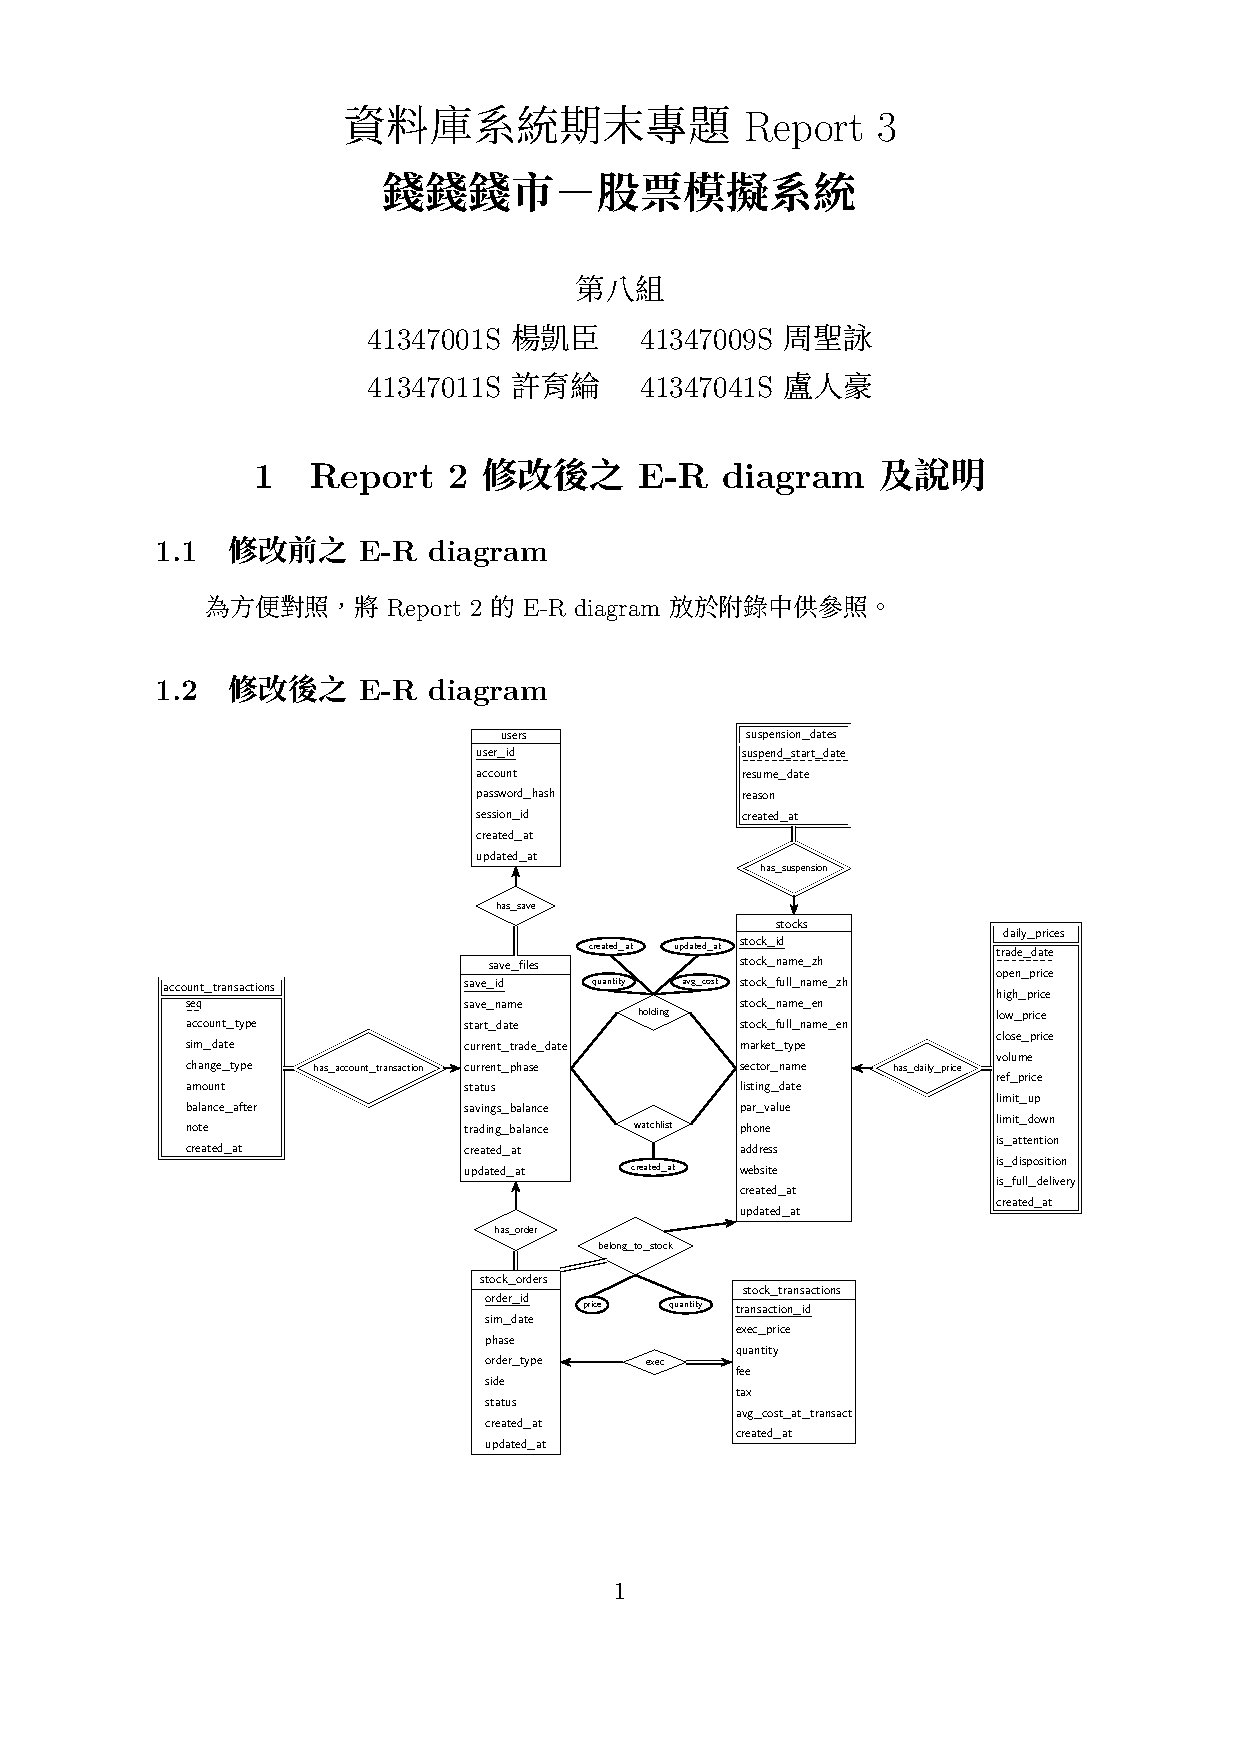
\includepdf[
    pages={-23}, 
    pagecommand={\thispagestyle{headings}}, 
    scale=0.99, 
    offset=0 -0cm % 調整 PDF 位置以避免蓋住標題
]{../report3/report3.pdf}

\end{document}